\documentclass[10pt,twoside]{tesisIER}

\usepackage{hhline}					% para dibujar lineas
\usepackage{fancyheadings}				% este lo necesita el estilo tesisIER.cls
\usepackage{blindtext}            % Dummy text

\usepackage{hyperref}   % Hipervinculos
\usepackage{pdflscape} %  para rotar páginas
\usepackage{longtable} % or {lscape}
\usepackage[activeacute,spanish]{babel}

%%	CAMBIO A MEXICANO

\addto\captionsspanish{\renewcommand{\contentsname}{Contenido}}
\addto\captionsspanish{\renewcommand{\listfigurename}{Lista de Figuras}}
\addto\captionsspanish{\renewcommand{\listtablename}{Lista de Tablas}}
\addto\captionsspanish{\renewcommand{\tablename}{Tabla}}


%%	HEADERS
\pagestyle{fancyplain}
\renewcommand{\chaptermark}[1]{\markboth{#1}{}}
\renewcommand{\sectionmark}[1]{\markright{\thesection\, #1}}
\lhead[\fancyplain{}{\bfseries\thepage}]%
      {\fancyplain{}{\bfseries\rightmark}}
\rhead[\fancyplain{\leftmark}{\bfseries\leftmark}]%
      {\fancyplain{}{\bfseries\thepage}}
\cfoot[]{}





%%	VECTORES
\newcommand{\vc}{\textbf c}
\newcommand{\BPSP}{\begin{pspicture}}
\newcommand{\EPSP}{\end{pspicture}}
\newcommand{\vF}{\textbf F}
\newcommand{\vg}{\textbf g}
\newcommand{\vG}{\textbf G}
\newcommand{\vn}{\textbf n}
\newcommand{\vN}{\textbf N}
\newcommand{\vPi}{\textbf \Pi}
\newcommand{\vq}{\textbf q}
\newcommand{\vr}{\textbf r}
\newcommand{\vu}{\textbf u}
\newcommand{\vv}{\textbf v}
\newcommand{\vU}{\textbf U}
\newcommand{\BE}{\begin{equation}}
\newcommand{\EE}{\end{equation}}

%%	VARIOS
\newcommand{\PROM}[1]{\left\langle #1\right\rangle}
\newcommand{\lsim}{\mathrel{\hbox{\rlap{\lower.55ex\hbox{$\sim$}} \kern-.3em 
 \raise.4ex \hbox{$<$}}}}




%%	PATH FIGURAS
\graphicspath{{figuras/}}  %define el subdirectorio donde latex busca las figuras, se pueden definir varios\usepackage{times}\renewcommand{\familydefault}{cmss}   % cambia el tipo de letra
%\usepackage{cite}                                      % se usa para la bibliograf'ia este no lo usa ulises
\usepackage[spanish,activeacute]{babel}				% este es el delos acentos as'i
\usepackage[utf8]{inputenc}				% este es el delos acentos normales así
\usepackage{amsmath}					% fonts m'as bonitas en las ecuaciones
%\usepackage{natbib}					% es el mero mero para la bibliografia
\usepackage{appendix}					% te permite usar ap'endices
\usepackage{amsfonts}					% m'as fonts
\usepackage{graphicx}				% include figures 
\usepackage{color}					% para definir colores
\usepackage{colortbl}					% m'as colores



%%	VARIOS

\title{Mi tesis en \LaTeX sin sufrir$^{\text{mucho}}$ en el proceso}
\author{Guillermo Barrios del Valle}

%\includeonly{resumen}
%\includeonly{introduccion}
%\includeonly{ebrv2}
%\includeonly{experimentosv2}
%\includeonly{conclusiones}
%\includeonly{validacion}



\begin{document} 
%
\spanishdecimal{.}
%
%\thispagestyle{empty}

\begin{pspicture}(13,19)
%\psgrid
\rput[C](1.1,17.3){\includegraphics[width=2.cm]{logo-unam.eps}}
\rput[C](1.1,.8){\includegraphics[width=2.cm]{logo-cie.eps}}
\psline[linewidth=0.2mm](2.2,17.2)(13,17.2)
\psline[linewidth=0.8mm](2.2,17.1)(13,17.1)
\rput[C](7.55,18.){ {\large\textbf{UNIVERSIDAD NACIONAL AUT\'ONOMA DE M\'EXICO}}}
\psline[linewidth=0.2mm](1,16)(1,1.4)
\psline[linewidth=0.8mm](0.8,16)(0.8,2)
\psline[linewidth=0.8mm](1.2,16)(1.2,2)

\rput[C](7.1,16.8){{\textbf{PROGRAMA DE MAESTR\'IA Y DOCTORADO EN}}}
\rput[C](7.1,16.3){{\textbf{INGENIER\'IA}}}


\rput[C](7.1,14.8){{{FACULTAD DE INGENIER\'IA}}}

\rput[C](7.1,12){{\textbf{LEVITACI\'ON DE PART\'ICULAS}}}
\rput[C](7.1,11.6){{\textbf{EN ONDAS DE SONIDO}}}
\rput[C](7.1,11.2){{\textbf{USANDO EL M\'ETODO DE LA}}}
\rput[C](7.1,10.8){{\textbf{ECUACI\'ON DE BOLTZMANN EN REDES }}}



\rput[C](7.1,9){{\textbf{T E S I S}}}

\rput[C](7.1,8){{QUE PARA OPTAR POR EL GRADO DE:}}

\rput[C](7.1,7){{\textbf{DOCTOR EN INGENIER\'IA}}}
\rput[C](7.1,6.5){{\textbf{\'AREA  MEC\'ANICA}}}
\rput[C](7.1,6){{\textbf{OPCI\'ON TERMOFLUIDOS}}}

\rput[C](7.1,5){ {P R E S E N T A : }}
\rput[C](7.1,4.5){{\textbf{M. I. GUILLERMO BARRIOS DEL VALLE}}}

\rput[C](7.1,3.5){ {T U T O R : }}
\rput[C](7.1,3){{\textbf{DR. RA\'UL RECHTMAN SCHRENZEL}}}

\rput[C](7.1,2){ {AGOSTO 2007 }}

\end{pspicture}

\newpage
\thispagestyle{empty}


{\textbf JURADO ASIGNADO:}
\vspace{1cm}

Presidente: Dr. Jaime Cervantes de Gortari
\vspace{0.5cm}

Secretario: Dr. Jorge Antonio Rojas Men'endez
\vspace{0.5cm}

1er Vocal:  Dr. Ra'ul Mauricio Rechtman Schrenzel
\vspace{0.5cm}

2do Vocal:  Dr. H'ector Lorenzo Ju'arez Valencia
\vspace{0.5cm}

3er Vocal:  Dr. Francisco Javier Solorio Ordaz
\vspace{1cm}

Centro de Investigaci'on en Energ'ia, Temixco, Morelos, M'exico.
\vspace{1cm}

{\textbf TUTOR DE TESIS:}
\vspace{1cm}

Dr. Ra'ul Rechtman Schrenzel










% 
%
\frontmatter
%
\chapter*{}
\thispagestyle{empty}


\begin{center}
A la comunidad  de software libre
\end{center}

\newpage
\thispagestyle{empty}
\chapter*{Agradecimientos}

Definitivamente este documento no hubiera sido posible sin  Raúl Rechtman (mi asesor durante mi maestría y doctorado, y ahora un gran amigo) quién me puso tres reglas al iniciar a trabajar con él: Programar en C, escribir en \LaTeX y graficar en Gnuplot.
%
\tableofcontents
%
\listoffigures
%


\chapter{Resumen}

En este documento encontraras los mejores consejos para que escribas
tu tesis en \LaTeX sin morir en el intento, sufrir es inevitable, pero la gloria
de una tesis linda te espera del otro lado del camino. Este documento es el resultado
 de más de 20 años de uso y revisión de documentos.

\newpage
\thispagestyle{empty}

\chapter{Abstract}
 
In this document i will try to give you my best advices for writting
your thesis in \LaTeX.

\newpage
\thispagestyle{empty}

%
\mainmatter
\chapter{Introducción}
\label{chap:introduccion}

 
 
 \section{Introducción}


Este documento reune mi experiencia en \LaTeX desde el 2001 conocí Linux y el software libre. Además, espero se enriquezca con las peticiones que se hagan al autor por medio de GitHub, correo electrónico.

En el Capítulo~\ref{chap:escritura} veremos como escribir secciones, subsecciones,  referencias a capítulos o secciones, citas con bibtex, ecuaciones, listas y tablas.

En el Capítulo~\ref{chap:figuras} será sobre las diferentes formas de incluir esquemas y figuras.

Dado que ahora muchos se han mudado a Overleaf, en el Apéndice~\ref{chap:overleaf} encontrarán las recomendaciones para trabajar en esa plataforma.


Recuerda revisar el código fuente para ver  como se hacen las cosas, descarga, comparte, comenta y te invito a hacer una contribución a este proyecto.

\chapter{Escritura}
\label{chap:escritura}


\section{Introducción}





En este capítulo explicaremos cada parte del estilo usado para esta plantilla en la sección~\ref{sec:cls},  como escribir secciones, subsecciones,  referencias a capítulos o secciones, citas con bibtex, ecuaciones, listas y tablas.


\section{tesisIER.cls}
\label{sec:cls}

En latex se define el tipo de documento al iniciar en 
\begin{verbatim} \documentclass[]{article} 
\end{verbatim}
y si te fijas, estamos usando un archivo tesisIER.cls que está basado en la book.cls.



\section{Estructura de archivos}


\section{Secciones y subsecciones}
\label{sec:secciones}

Esta es una sección.
\subsection{Esta es una subsección}
 A manera personal no recomiendo usar más allá de subsections.

\subsubsection{Sub sub sección}
A partir de este nivel, Latex automáticamente deja de numerar y tampoco aparecerán en el índice.



\section{Ecuaciones}

Un estilo para escribir ecuaciones, es considerarlas como texto, entonces, la ecuación de aceleración es
\begin{equation}
a  = \frac{dv}{dt},
\label{eq:aceleracion}
\end{equation}
donde $a$ es la aceleración [$m/s^2$], $v$ es la velocidad [$m/s$] y $t$ el tiempo [$s$]. Nota que no hay un renglón vacio entre la ecuación y la continuación del texto, de esa manera no aparecerá una sangría donde no la quieres.

En la Ec.~\ref{eq:aceleracion} estamos presentando la definición de la aceleración, y te recominedo usar etiquetas agregando algo que te de referencia a lo que es, una tabla (table:palabra), ecuación (eq:palabra), figura (fig:palabra) donde la palabra describe la ecuación, de esa manera, cuando el programa que usas autocomplete y tengas una lista interminable, te será más fácil identificar la etiqueta adecuada.

\section{Tablas}
\label{sec:tablas}

Las tablas pueden causar dolores de cabeza, especialmente cuando son muy largas, y un editor de LaTeX se agradece para crearlas. Una tabla sencilla es la mostrada en~\ref{tabla:sencilla}.

\begin{table}
\centering
\begin{tabular}{lcr}
Item                    &    Cantidad    & Precio \\
                          &    [-]              & [mxn]  \\
\hline
\hline
bolsa croquetas  &    1               & 999.99 \\
jabon platos       &    1               & 9.99 \\
\hline
\hline
\end{tabular}
\caption{ Esta es mi lista de super de hoy.
\label{tabla:sencilla}
}
\end{table}

La clave para escribir tablas como la mostrada en~\ref{tabla:sencilla} es que desde tu editor de texto la puedas ver estructurada, as\'i ser\'a m\'as f\'acil ver los errores. Como puedes ver, LaTeX tambi\'ien decide donde poner las tablas, te recomiendo no forzar nada. No olvides agregar un rengl\'on para las unidades.



Si tienes una tabla muy larga como la Tabla~\ref{tabla:larga} , donde se decidió rotar una página para insertarla y que se pueda usar esta página en modo apaisado. No te recomiendo achicar la tabla, habemos quienes sufrimos mucho con la letra chiquita. Para rotar la página se utiliza el paquete landscape y se pone en un ambiente lo que se desea poner en la página o páginas rotadas.


\begin{landscape}
\begin{table}
\centering
\begin{tabular}{lcrl}
Item                    &    Cantidad    & Precio  & Descripci\'on  \\
                          &    [-]              & [mxn]   &                       \\
\hline
\hline
bolsa croquetas  &    1               & 999.99  & Esta es una descripci\'on muy larga para hacer una prueba de una tabla larga\\
jabon platos       &    1               & 9.99      &  Esta es una descripci\'on muy larga para hacer una prueba de una tabla larga\\
\hline
\hline
\end{tabular}
\caption{ Esta es una  lista muy larga de ejemplo en una página rotada.
\label{tabla:larga}
}
\end{table}
\end{landscape}


Puede ser que tengan una tabla tan larga, Tabla~\ref{tabla:dospaginas} que requieras más de una página, para esos casos usa el ambiente longtable que lo proporciona el paquete con el mismo nombre.

\begin{longtable}{lcr}
Item                   &    Cantidad    & Precio \\
                          &    [-]              & [mxn]  \\
\hline
\hline
bolsa croquetas  &    1               & 999.99 \\
jabon platos       &    1               & 9.99 \\
bolsa croquetas  &    1               & 999.99 \\
jabon platos       &    1               & 9.99 \\
bolsa croquetas  &    1               & 999.99 \\
jabon platos       &    1               & 9.99 \\
bolsa croquetas  &    1               & 999.99 \\
jabon platos       &    1               & 9.99 \\
bolsa croquetas  &    1               & 999.99 \\
jabon platos       &    1               & 9.99 \\
bolsa croquetas  &    1               & 999.99 \\
jabon platos       &    1               & 9.99 \\
bolsa croquetas  &    1               & 999.99 \\
jabon platos       &    1               & 9.99 \\
bolsa croquetas  &    1               & 999.99 \\
jabon platos       &    1               & 9.99 \\
bolsa croquetas  &    1               & 999.99 \\
jabon platos       &    1               & 9.99 \\
bolsa croquetas  &    1               & 999.99 \\
jabon platos       &    1               & 9.99 \\
bolsa croquetas  &    1               & 999.99 \\
jabon platos       &    1               & 9.99 \\
bolsa croquetas  &    1               & 999.99 \\
jabon platos       &    1               & 9.99 \\
bolsa croquetas  &    1               & 999.99 \\
jabon platos       &    1               & 9.99 \\
bolsa croquetas  &    1               & 999.99 \\
jabon platos       &    1               & 9.99 \\
bolsa croquetas  &    1               & 999.99 \\
jabon platos       &    1               & 9.99 \\
bolsa croquetas  &    1               & 999.99 \\
jabon platos       &    1               & 9.99 \\
bolsa croquetas  &    1               & 999.99 \\
jabon platos       &    1               & 9.99 \\
bolsa croquetas  &    1               & 999.99 \\
jabon platos       &    1               & 9.99 \\
bolsa croquetas  &    1               & 999.99 \\
jabon platos       &    1               & 9.99 \\
bolsa croquetas  &    1               & 999.99 \\
jabon platos       &    1               & 9.99 \\
bolsa croquetas  &    1               & 999.99 \\
jabon platos       &    1               & 9.99 \\
bolsa croquetas  &    1               & 999.99 \\
jabon platos       &    1               & 9.99 \\
bolsa croquetas  &    1               & 999.99 \\
jabon platos       &    1               & 9.99 \\
bolsa croquetas  &    1               & 999.99 \\
jabon platos       &    1               & 9.99 \\
bolsa croquetas  &    1               & 999.99 \\
jabon platos       &    1               & 9.99 \\
bolsa croquetas  &    1               & 999.99 \\
jabon platos       &    1               & 9.99 \\
bolsa croquetas  &    1               & 999.99 \\
jabon platos       &    1               & 9.99 \\
bolsa croquetas  &    1               & 999.99 \\
jabon platos       &    1               & 9.99 \\
bolsa croquetas  &    1               & 999.99 \\
jabon platos       &    1               & 9.99 \\
\hline
\hline
%\end{tabular}
\caption{ Esta es mi lista de super de hoy.
\label{tabla:dospaginas}
}
\end{longtable}



\section{Bibtex y yo}


Lo ideal es que uses bibtex para administrar tus citas, te recomiendo que revises el archivo bibliografia.bib y uses un editor de \LaTeX para poder agregar campos bibliográficos con un simple botonazo. Para citar correctamente hay que usar la tilde pegada a la última palabra~\cite{he97}. De esa manera, la cita y la última palabra forman un bloque y el paquete hyphenation no las separa de ser necesario, además da una separación muy linda visualmente.  Recuerda que puedes citar muchos autores al mismo tiempo y bibtex los va acomodar~\cite{ansumali00,buick98,buick98a,guo00}. Todos los anteriores hicieron trabajos sobre levitación acústica, por si te da curiosidad saber quienes son.



\subsection{Compilando con bibtex y más}

Recuerda correr pdflatex y luego bibtex y luego otra vez dos veces pdflatex para que los cambios en tu bibliografía se vean reflejados.  Esto es necesario porque en la primer compilación de pdflatex se crea el archivo bbl y luego se actualiza en la segunda compilación.

Si quieres comenzar un nuevo párrafo,  solo debes dejar una línea y el párrafo nuevo se distingue por la sangría, no uses doble diagonal para poner un espacio extra, esa es una mala práctica.



Por cierto, si notas que los margenes están desiguales, es por qué esta tesis está configurada para imprimirse por los dos lados, cuando las tesis tenían que ser impresas a fuerza, eso lo puedes desactivar en el preambulo de main.tex, actualmente está
\begin{verbatim}
\documentclass[10pt,twoside]{tesisIER}
\end{verbatim}
y lo puedes arreglar usando:
\begin{verbatim}
\documentclass[10pt,oneside]{tesisIER}
\end{verbatim}
para que no se vea con los margenes desiguales. Es importante seleccionar el twoside si imprimes por los dos lados de la hoja. 

\section{Editores de \LaTeX}
\subsection{TexMaker}
\subsection{Emacs}
\subsection{Vim}


\subsection{\LaTeX y Python, la vida es bella}


\section{Conclusiones}


\chapter{Figuras}
\label{chap:figuras}


 
 
 \section{Tipos de figuras y sus editores}
\subsection{Configuración de ambiente y posicionamiento}
 En la Figura~\ref{fig:IER} se muestra una captura de la página web del IER-UNAM.
 \begin{figure}
 \centering
 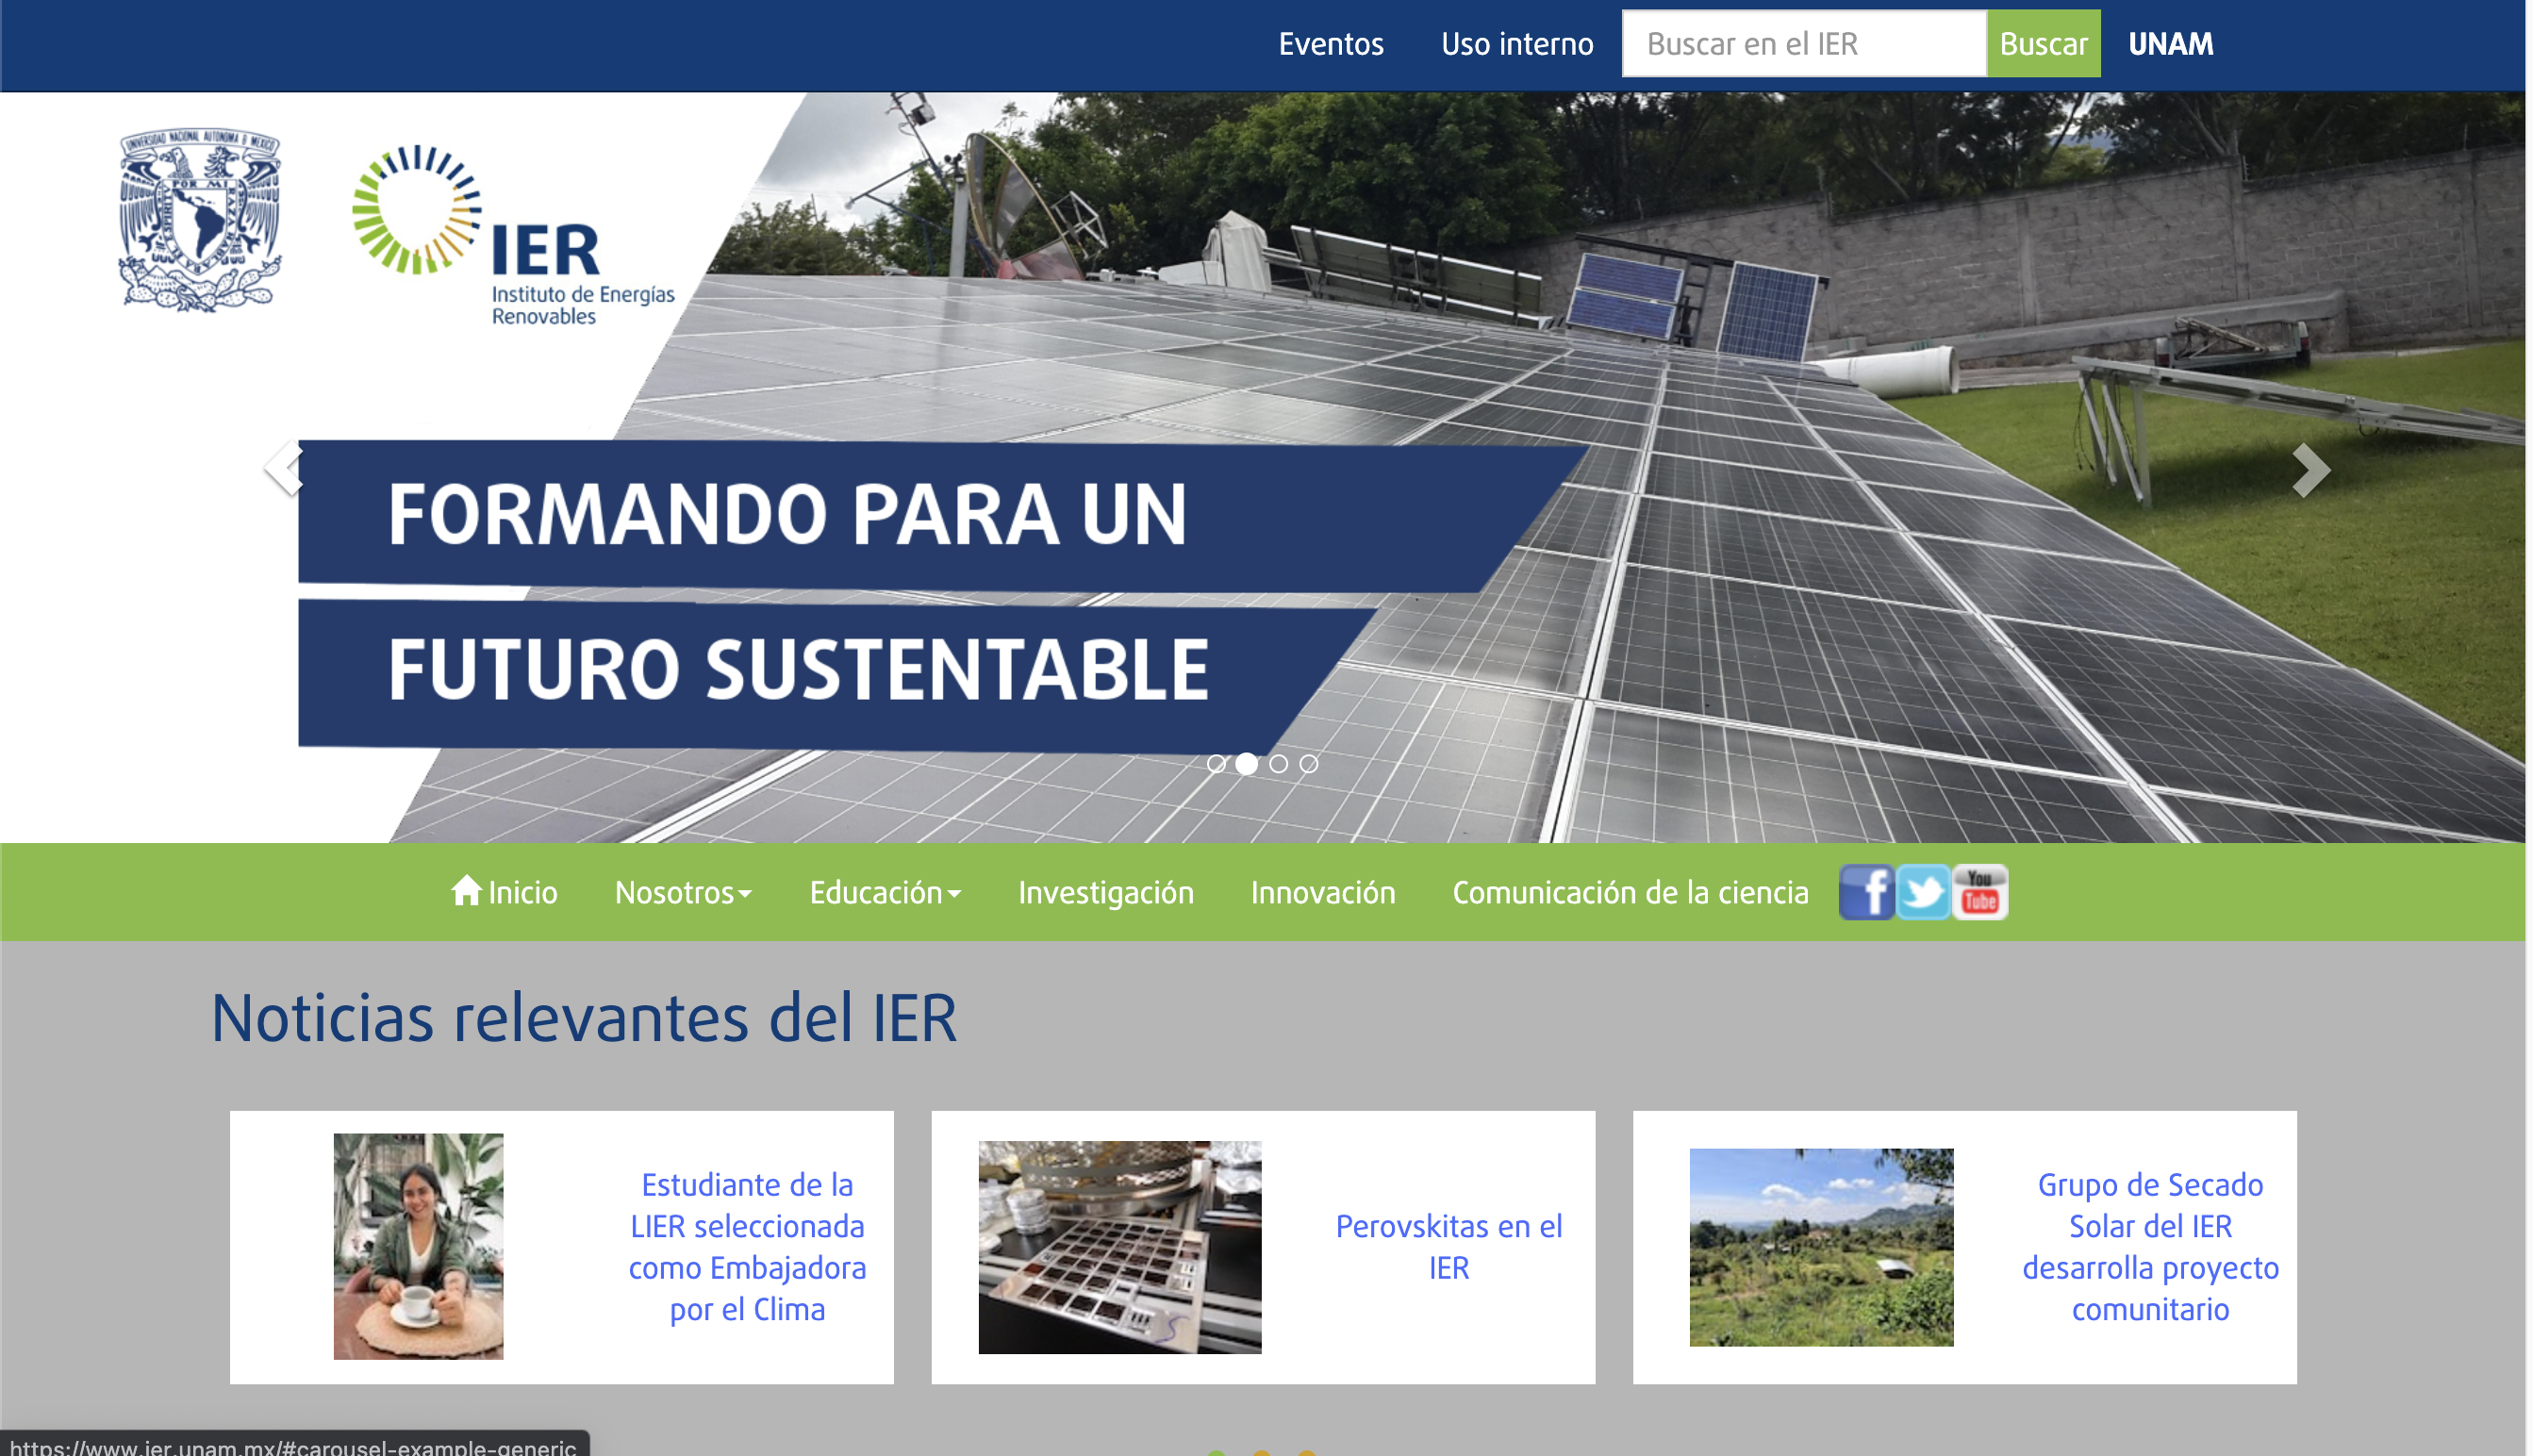
\includegraphics[scale=0.2]{ier_homepage}
 \caption{	
 Captura tomada de la página web del IER-UNAM.
 \label{fig:IER}
 }
 \end{figure}
 
 La figura se incluyó con el siguiente código
 \begin{verbatim}
 \begin{figure}
 \centering
 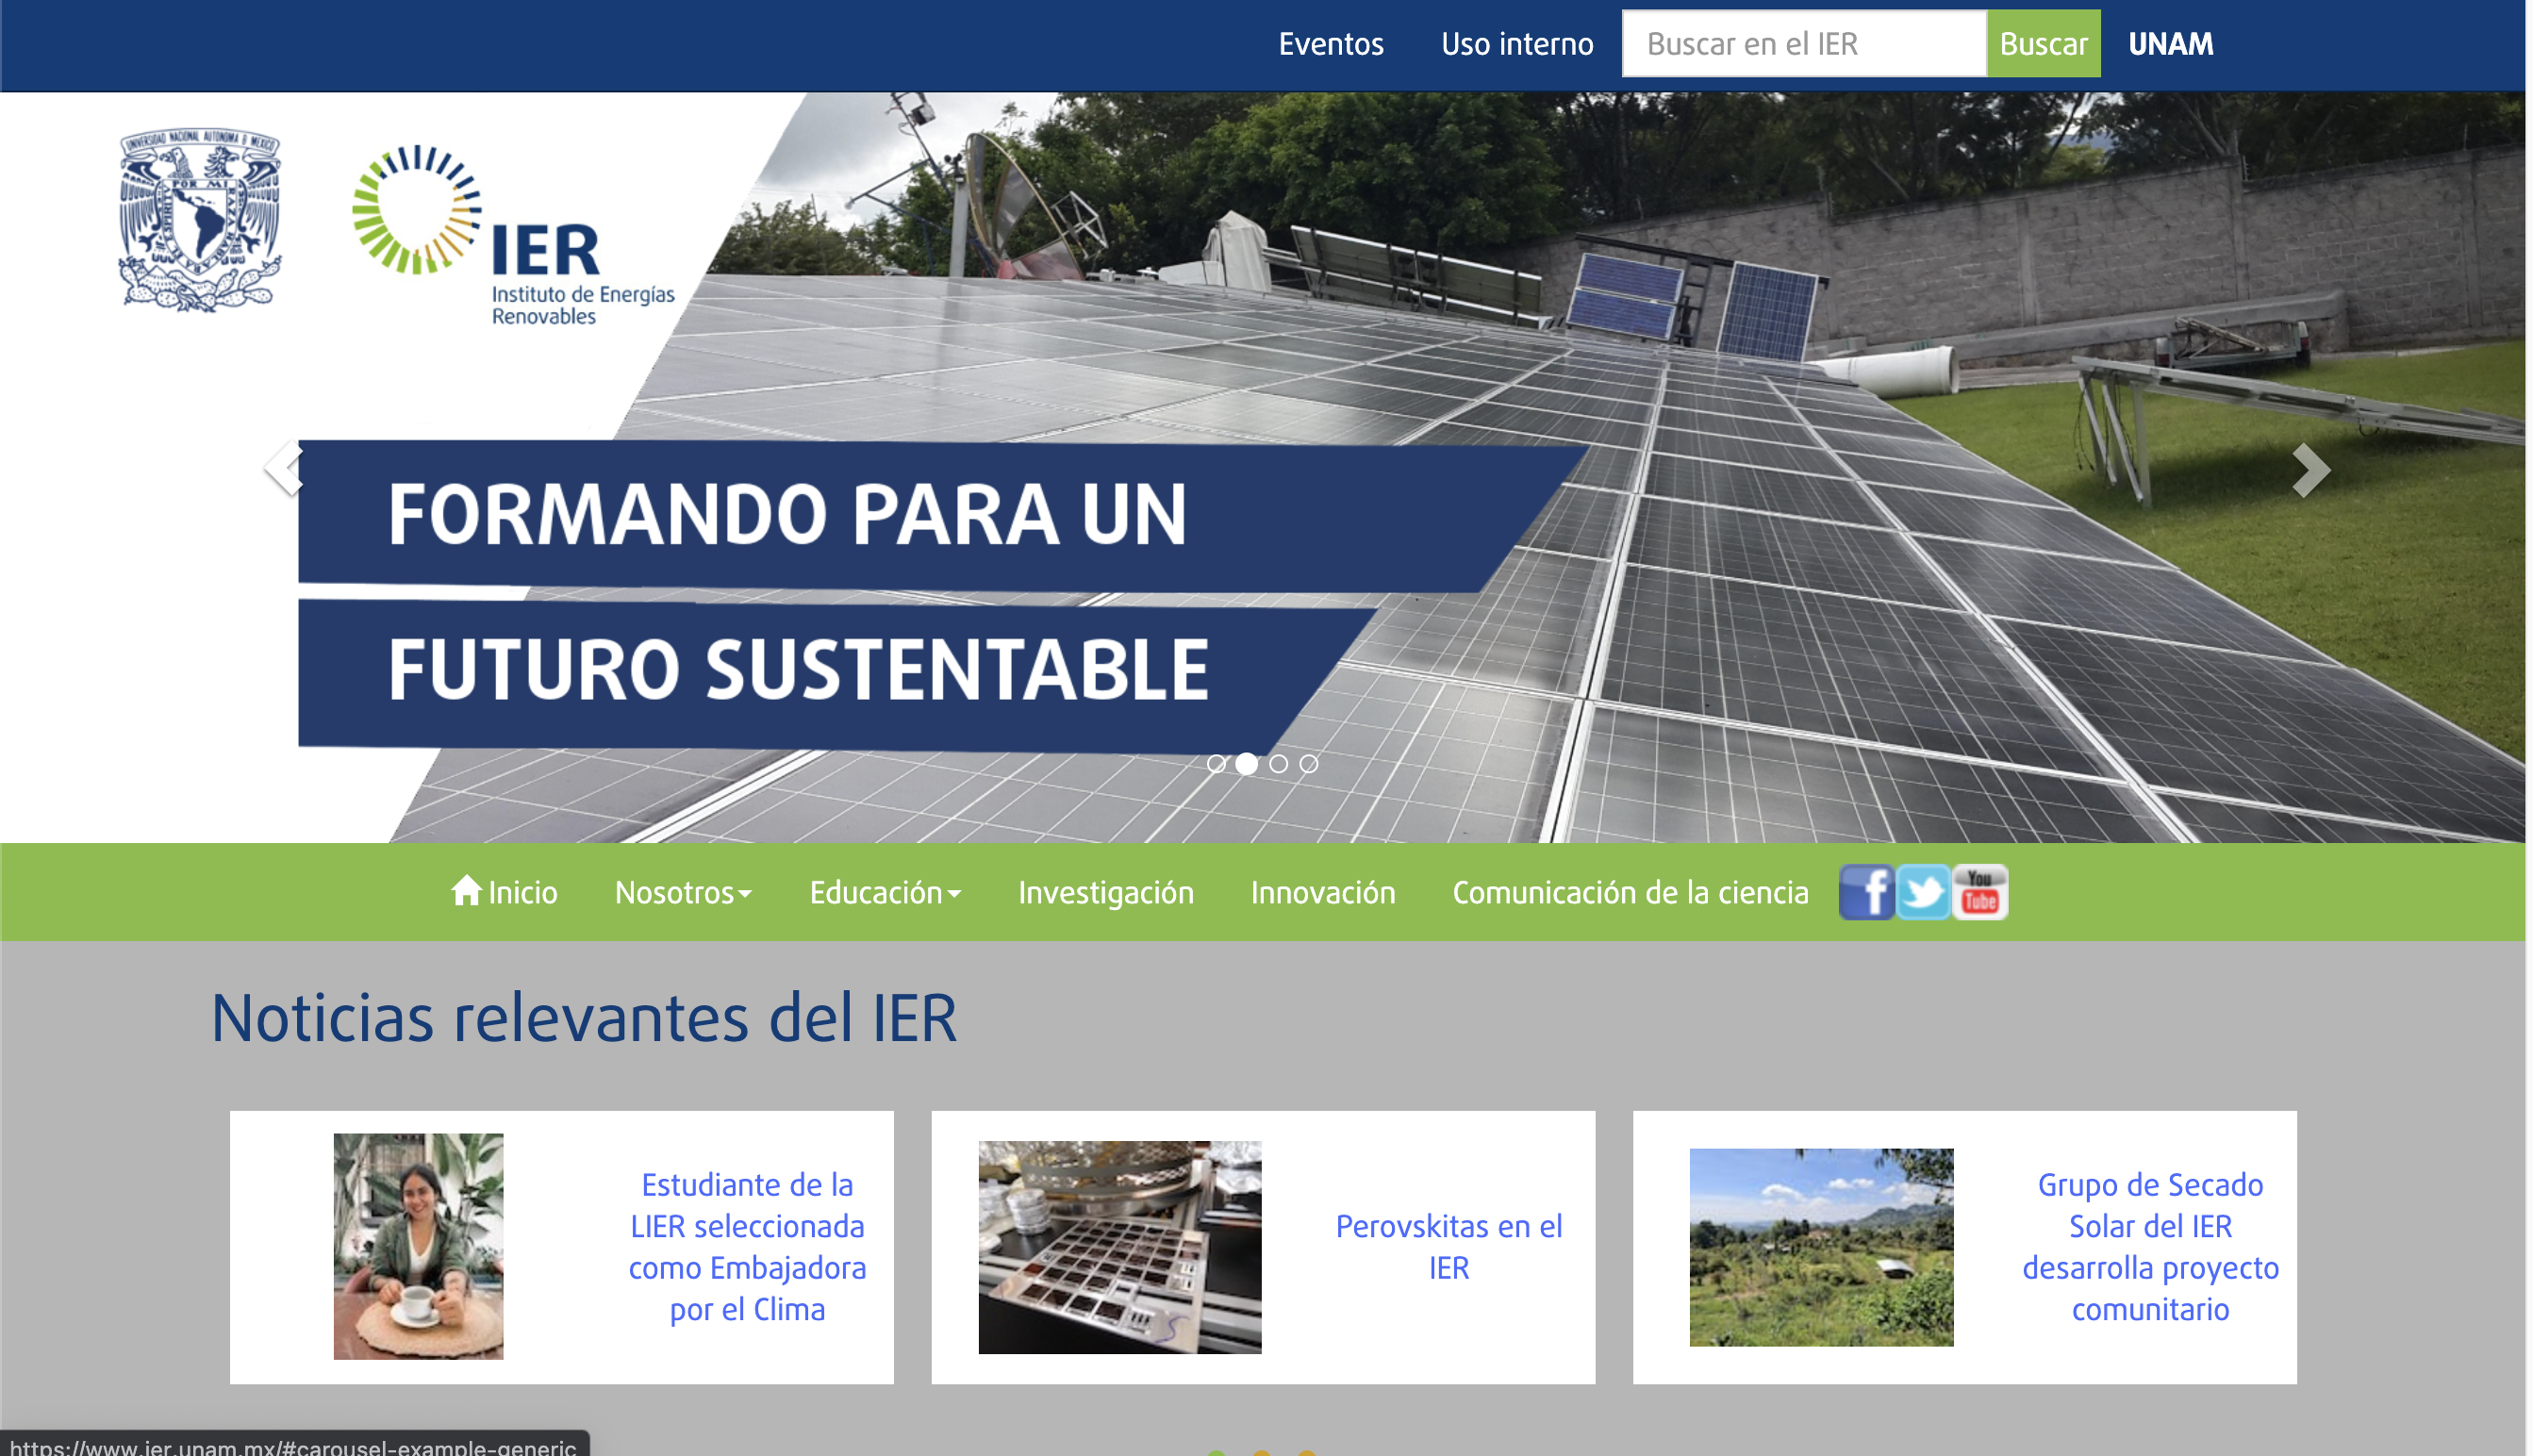
\includegraphics[scale=0.2]{ier_homepage}
 \caption{	
 Captura tomada de la página web del IER-UNAM.
 \label{fig:IER}}
 \end{figure}
 \end{verbatim}
 
Una práctica muy común que veo es que usan 
 \begin{verbatim}
 \begin{figure}[!ht]
 \end{verbatim}
 que le está diciendo a latex forzar a poner la figura en la misma página que el texto y en la parte superior de la página. Te recomiendo no usar esto y darle oportunidad a latex de acomodar las figuras de acuerdo a su criterio, además conforme tengas más texto, las figuras irán cambiando su lugar y se verá mejor.
\subsection{Figuras en pdf}
\subsection{Figuras en png/jpg}
\subsection{Figuras en epslatex}
\subsection{Figuras con gnuplot}
\subsection{Figuras en tex}
\subsection{Recomendaciones generales}
%\include{capitulos/experimentosv2}
%\include{capitulos/conclusiones}
%
%
\appendix
\chapter{Overleaf}
\label{chap:overleaf}

 
 
 \section{Introducción}

%
%
\backmatter
\bibliographystyle{unsrt} %unsrt,alpha,abbrv,plain
\bibliography{bibliografia}
%
%
\end{document}
